\documentclass[10pt,a4j]{ltjsarticle}

% 卒業研究報告書スタイルファイル
\usepackage{layouts/tsuyama/eeses}

% ソースコード表示
\usepackage{listings}
% 色
\usepackage{xcolor}
% 数学関連
\usepackage{amsmath, amssymb}
% リスト制御
\usepackage{enumitem}
% newtxフォント
\usepackage{newtxmath, newtxtext}
% 画像
\usepackage{graphicx}
% shaded環境の背景色の定義
\definecolor{shadecolor}{gray}{0.80}
% 枠
\usepackage{ascmac}
\usepackage{tcolorbox}
% url表記
\usepackage{url}
% ハイパーリンク
\usepackage[pdfencoding=auto]{hyperref}
% フォント
\usepackage{layouts/lualatexsets/fonts}
% Tikz関係
\usepackage{tikz}
% 証明などのスタイル
\usepackage{layouts/others/theorem}
% セクションの表示スタイル
%\usepackage{layouts/others/section}
% ベクトル表記
\usepackage{bm}
\def\vector#1{\mathop{\mathbf{#1}}}
% 疑似アルゴリズム
\usepackage{algorithm}
\usepackage{algorithmic}
% 画像・図表等のrefコマンド
\def\thmref#1{Thm. \ref{#1}}
\def\lmmref#1{Lemma. \ref{#1}}
\def\figref#1{図\ref{#1}}
\def\eqref#1{(\ref{#1})式}
\def\tableref#1{表\ref{#1}}

%%% ドキュメント情報 %%%
% 著者
\author{萩原 涼介}
% タイトル
\title{クラスタ数推定に用いる最適な情報量基準の探求}
% 指導教員
\adviser{藤田 一寿}
% 日付
\date{\today}
% 学科
\affiliation{情報}
% 種別
\kind{\midpre}
% pdfファイル情報
\hypersetup{%
  colorlinks=true,%
  urlcolor=black,%
  linkcolor=black,%
  citecolor=black,%
  linktocpage=true,%
  bookmarks=false,%
  pdftitle={卒業研究 中間報告書},%
  pdfsubject={クラスタ数推定に用いる最適な情報量基準の探求},%
  pdfauthor={Hagihara Ryosuke},%
  pdfkeywords={クラスタリング; 情報量規準; クラスタ数推定; 機械学習}
}


\begin{document}
\maketitle
\tableofcontents

% はじめに
\section{はじめに}
クラスタリングとはデータを教師なし学習により任意の数のクラスタに分ける手法である.
クラスタリングはデータ解析,データマイニング,パターン認識など様々な分野で用いられる.
K-meansを始めとする多くのクラスタリング手法では,予めクラスタ数がわかっているものとして,
クラスタ数を指定しクラスタリングを行う.
しかし,データに対し最適なクラスタ数を指定しなければ,最適なクラスタリング結果を得ることはできないが,
一般にクラスタ数が事前にわかっているデータは少ない.
その為,クラスタ数が未知である場合にも,適切にクラスタ数を推定することは重要な課題となっている.

既存の手法の多くは,データが確率分布関数から生成されたと想定して,
その確率分布を生成するモデルを推定することにより,クラスタ数推定を行う.
クラスタ数推定を行う際,よく用いられるのが情報量規準と呼ばれれる指標である.
情報量規準とは簡単に言えば確率分布とデータの分布の当てはまり具合を表す.
その情報量基準は多くの研究者により様々なものが提案されている.
例えば,1973年に赤池が提案したAIC (Akaike Information Criterion) や,
Bayesの定理によって算出される事後確率を用いるBIC (Bayesian Information Criterion)が有名である.

しかし,どの情報量規準がどのようなデータに対し有効かは分かっていない.
そこで本研究では,クラスタ数推定に用いる情報量規準として最適なものを数値実験を通し明らかにする.

前期は,混合等方Gauss分布から生成されたデータ,ランダムに生成されたデータおよび
自然のデータであるアヤメの形態などのデータと白ワインの品質に関するデータをX-meansにより
クラスタ数推定およびクラスタリングを行い,AIC, cAIC, BICと呼ばれる情報量規準によるクラスタリングの性能の評価を行った.

第2章では,既存のクラスタリング手法であるK-meansのアルゴリズムの紹介を行う.

第3章では,本研究で利用するX-meansの理論の説明を行う.
まず,モデルと真の確率分布との近さを計る指標であるKullback-Leibler情報量について述べ,
それと最尤推定との情報量規準の関係性について詳しく述べる.
その後,X-meansの手法について述べる.

第4章では,本研究により得られた実験結果について述べる.

第5章では,本研究を通してのまとめおよび今後の課題について述べる.

% 先行研究
\section{先行研究}

\subsection{クラスタリング}
クラスタリングとはデータを教師なし学習により任意の数のクラスタに分ける手法である.
クラスタとは,似ているデータの集まりである.
クラスタリング手法において,データの類似の度合いはユークリッド距離やコサイン距離などの距離尺度を用い計算する.
クラスタリングはデータ解析,データマイニング,画像処理,パターン認識など様々な分野で用いられる.

\subsection{$k$-means}
%k-meansのkは$k$
様々なクラスタリング手法の中で最も有名な手法が$k$-meansである.
$k$-means\cite{k-means}は,$d$次元空間上のデータについて,ユークリッド距離を用い各データ点が属するクラスタを決定する手法である.
% $k$-meansは,以下の2つの手順を繰り返すことでクラスタリングを行う.
% \begin{enumerate}
%   \item 各データ点とデータ点の距離を求め,各データ点を最も近いセントロイドのクラスタに割り当てる.
%   \item クラスタに所属するデータの平均を新たなセントロイドとする.
% \end{enumerate}
% セントロイドが移動しなくなったらクラスタリングを終了する.

$d$次元空間上の確率変数$\vector{x}$の$N$個のデータ点で構成されるデータ
$\{\vector{x}_1, \vector{x}_2, ..., \vector{x}_N\}$があるとする.
このデータを$K$個のクラスタに分割することを考える.
ここで,セントロイド$\vector{\mu}_k$を導入する.セントロイド$\vector{\mu}_k$とはクラスタ$k$の重心を表す.
$k$-meansはクラスタに所属するデータ点とそのクラスタのセントロイド間のユークリッド距離の総和を最小にすることで,クラスタリングを行う.

ここで,各データ点$\vector{x}_n$に対し,対応する2値指示変数$r_{nk} \in \{0, 1\}\ (k = 1, \cdots, K)$を定める.
これは,そのデータ点$\vector{x}_n$がクラスタ$k$に割り当てられるかを表す変数である.
すなわち,データ点$\vector{x}_n$がクラスタ$k$に割り当てられる場合は$r_{nk}=1$とし,
そうでない場合は$r_{nk}=0$とする.これは,1-of-K符号化法として知られている.

次に,$k$-meansにおける目的関数$J$を定義する.
\begin{align}
  \label{eq:J-func}
  J = \sum_{n=1}^{N} \sum_{k=1}^{K} r_{nk} \| {\displaystyle \vector{x}_n - \vector{\mu}_k} \|^2
\end{align}
これは,各データ点からそれらが割り当てられたクラスタのセントロイド$\vector{\mu}_k$までのユークリッド距離の2乗の総和を表している.%ユークリッド距離が嫌ならL2ノルム
$k$-meansによるクラスタリングは,$J$を最小にする$\{r_{nk}\}$と$\{\vector{\mu}_k\}$の値を求めることに換言できる.

まず$r_{nk}$の決定を考える.
\eqref{eq:J-func}における$J$は$r_{nk}$についての線形関数なので,最適化は代数的に解くことができる.
異なる$n$を含む項は互いに独立である.よって,各$n$について別々に$r_{nk}=1$としたときに,
$||\vector{x}_n - \vector{\mu}_k||^2$が最小になるような$k$の値に対して$r_{nk}$を選んで1とおけばよい(\eqref{eq:rnk}).
\begin{align}
  \label{eq:rnk}
  r_{nk} = \left\{
    \begin{array}{ll}
      1 & k = \arg\min_j \|\vector{x}_n - \vector{\mu}_j\|  \text{のとき}\\
      0 & \text{それ以外}
    \end{array}
  \right.
\end{align}
つまり,単純に$n$番目のデータ点がそれに最も近いセントロイドを持つクラスタに割り当てるのである.

次に,$r_{nk}$を固定したもとで$\vector{\mu}_k$の最適化を考える.
対象関数$J$は$\vector{\mu}_k$の二次関数であり,次のように$\vector{\mu}_k$に関する偏微分を0とおく事で最小化できる
(\eqref{eq:mu-dif}).
\begin{align}
  \label{eq:mu-dif}
  2\sum_{n=1}^n r_{nk}(\vector{x}_n - \vector{\mu}_k) = 0
\end{align}
これを$\vector{\mu}_k$についてとくと,\eqref{eq:mu}を得る.
\begin{align}
  \label{eq:mu}
  \vector{\mu}_k = \frac{\sum_n r_{nk}\vector{x}_n}{\sum_n r_{nk}}
\end{align}
この式の分母は$k$番目のクラスタに割り当てられたデータの数に等しい.
それゆえ$\vector{\mu}_k$は$k$番目のクラスタに割り当てられた全てのデータ点$\vector{x}_n$の
平均値と単純に解釈することができる.

\begin{figure}[htbp]
  \begin{minipage}{0.33\hsize}
    \begin{center}
      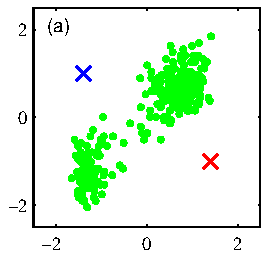
\includegraphics[width=40mm]{img/kmeans/Figure91a.pdf}
    \end{center}
  \end{minipage}
  \begin{minipage}{0.33\hsize}
    \begin{center}
      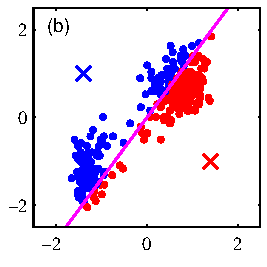
\includegraphics[width=40mm]{img/kmeans/Figure91b.pdf}
    \end{center}
  \end{minipage}
  \begin{minipage}{0.33\hsize}
    \begin{center}
      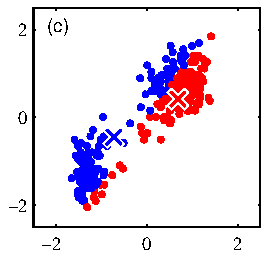
\includegraphics[width=40mm]{img/kmeans/Figure91c.pdf}
    \end{center}
  \end{minipage}\\
  \begin{minipage}{0.33\hsize}
    \begin{center}
      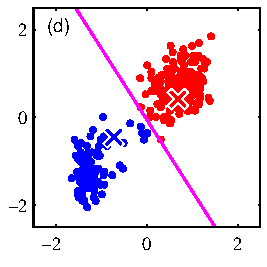
\includegraphics[width=40mm]{img/kmeans/Figure91d.pdf}
    \end{center}
  \end{minipage}
  \begin{minipage}{0.33\hsize}
    \begin{center}
      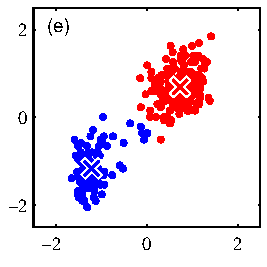
\includegraphics[width=40mm]{img/kmeans/Figure91e.pdf}
    \end{center}
  \end{minipage}
  \begin{minipage}{0.33\hsize}
    \begin{center}
      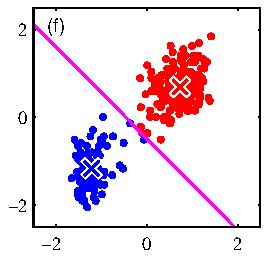
\includegraphics[width=40mm]{img/kmeans/Figure91f.pdf}
    \end{center}
  \end{minipage}\\
  \begin{minipage}{0.33\hsize}
    \begin{center}
      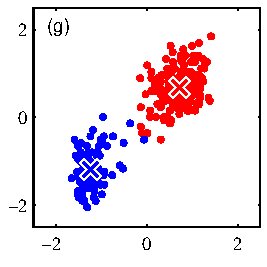
\includegraphics[width=40mm]{img/kmeans/Figure91g.pdf}
    \end{center}
  \end{minipage}
  \begin{minipage}{0.33\hsize}
    \begin{center}
      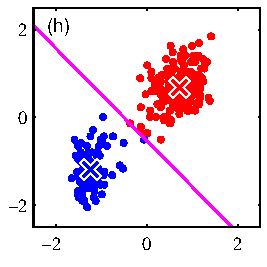
\includegraphics[width=40mm]{img/kmeans/Figure91h.pdf}
    \end{center}
  \end{minipage}
  \begin{minipage}{0.33\hsize}
    \begin{center}
      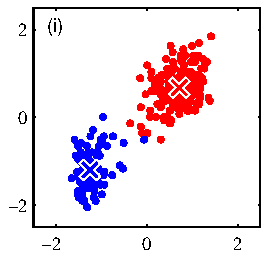
\includegraphics[width=40mm]{img/kmeans/Figure91i.pdf}
    \end{center}
  \end{minipage}
  \caption{$k$-meansの動作}
  \label{fig:k-means}
\end{figure}

\figurenum{fig:k-means}に$k$-meansによるクラスタリングの具体例を示す.
$k$-meansでは,$r_{nk}$と$\vector{\mu}_k$をそれぞれ最適化する2つのステップを
交互に繰り返す手続きでクラスタリングを実現する.
最初に,$\vector{\mu}_k$の初期値を選ぶ(\figurenum{fig:k-means}a).
次に,最初のフェーズで$\vector{\mu}_k$を固定しつつ,$r_{nk}$について$J$を最小化する(\figurenum{fig:k-means}b).
第二フェーズでは,$r_{nk}$を固定しつつ,$\vector{\mu}_k$について$J$を最小化する(\figurenum{fig:k-means}c).
そして,このような二段階最適化を収束するように繰り返す.

データ点のクラスタへの再割り当てと,クラスタ平均の再計算という2つのフェーズは,
再割当てが起こらなくなるまで(もしくはあらかじめ定めた最大繰り返し数を超えるまで)繰り返される.
各フェーズは,対象関数$J$の値を減少させるので,このアルゴリズムの収束は保証されている.
しかしながら,大域的最小点ではなく極小点に収束する可能性はある.

なお,$k$-meansによるクラスタリングは,事前にクラスタ数を指定することによりクラスタリングを行うため
クラスタ数が未知の場合,$k$-meansを用いることはできない.

\subsection{Kullback-Leibler情報量}
偶然を伴う現象は,ある確率分布に従う確率変数の実現値であると考えることができる.
この確率分布を近似するモデル(以後「モデル」)は,データを生成する真の確率分布に
どの程度近いかによって評価することができる.
また,データにモデルを当てはめることは,データから真の確率分布を推定しているものと
みなすことができる.このようにモデルと真の分布が共に確率分布であると見なし,
モデルの評価や推定を行う.

真の分布とモデルの近さを測る客観的な規準としてKullback-Leibler情報量(以後「K-L情報量」)がある.
連続型の確率分布のとき,$g(x)$を真の確率密度関数,$f(x)$をモデルが定める確率密度関数とすると,
モデルに関する真の分布のK-L情報量は$\log\{g(X)/f(X)\}$の期待値を取り\eqref{eq:k-l-div}で表される.
\begin{align}
  \label{eq:k-l-div}
  I(g \mid f) &= \int^{\infty}_{-\infty}\log\left\{\frac{g(x)}{f(x)}\right\}g(x)dx
\end{align}
ただし,$\log$は自然対数で,注記がない限り一貫してこの意味で用いる.

このように,真の分布がわかっている場合にはK-L情報量によってモデルの良し悪しを比較できた.
しかし,通常は真の分布が未知で,真の分布から得られたデータだけが与えられていることが多い.
したがって,データからK-L情報量を推定する必要がある.
\eqref{eq:k-l-div}を展開すると
\begin{align}
  I(g \mid f) &= \int^{\infty}_{-\infty}\left\{\log\frac{g(x)}{f(x)}\right\}g(x)dx\\\nonumber
              &= -\int^{\infty}_{-\infty}\{\log f(x)\}g(x)dx - 
                 \left(-\int^{\infty}_{-\infty}\{\log g(x)\}g(x)dx\right)
\end{align}
となるが,右辺の第2項は定数であり,右辺第1項が大きいほどK-L情報量$I(g \mid f)$は
小さくなることがわかる.
すなわち,K-L情報量の大小比較のためには,本質的には$\int^{\infty}_{-\infty}\{\log f(x)\}g(x)dx$だけを推定すれば良いことがわかる.
右辺第1項の$\int^{\infty}_{-\infty}\{\log f(x)\}g(x)dx$は,確率密度関数$\log f(x)$の期待値であり,平均対数尤度と呼ばれている.
ここで,
\begin{align}
  \sum_{i=1}^{n}\log f(x_i)
\end{align}
を対数尤度と呼ぶことにすると,$n$個の独立な観測値$\{x_1, x_2, \cdots, x_i\}$が得られると,
この平均対数尤度は,対数尤度の$n$分の1
\begin{align}
  \frac{1}{n}\sum_{i=1}^{n}\log f(x_i)
\end{align}
で近似される.
したがって,符号に注意すると,対数尤度が大きいほど,そのモデルは真の分布に近いと考えられる.
このようにして,対数尤度をK-L情報量の推定値と考えることにすると異なったタイプのモデルの
良し悪しも比較できるのである.

ところで,確率変数$(X_1, X_2, \cdots, X_n)$の同時密度関数が$f(x_1, x_2, \cdots, x_n \mid \theta)$で
与えられているものとする.
$\theta$は確率密度関数を規定するパラメータである.この時,観測値$(x_1, x_2, \cdots, x_n)$は
与えられたものとして固定し,$f$を$\theta$の関数と考える時,この関数を\textbf{尤度}と呼び,
$L(\theta)$で表す.すなわち,
\begin{align}
  L(\theta) = f(x_1, x_2, \cdots, x_n \mid \theta)
\end{align}
である.特に,確率変数が独立な場合には$(X_1, X_2, \cdots, X_n)$の確率密度関数は,
各$X_i (i = 1, \cdots, n)$の確率密度関数の積に等しいことから,
\begin{align}
  L(\theta) &= f(x_1 \mid \theta)f(x_2 \mid \theta) \cdots f(x_n \mid \theta)\\\nonumber
  &= \prod_{i=1}^{n}f(x_i \mid \theta)
\end{align}
となる.この両辺の対数をとると,すでに求められた対数尤度関数
\begin{align}
  l(\theta) = \sum_{i=1}^{n}\log f(x_i \mid \theta)
\end{align}
が導かれる.

ここでは,平均対数尤度の推定量から対数尤度を直接導入した.
しかし,モデルが確率分布の形で与えられている場合には,まず観測値の同時分布から
尤度を定義し,その対数として対数尤度を求めるほうが都合が良い.
$(X_1, X_2, \cdots, X_n)$が独立でない場合にも,尤度の対数として対数尤度
\begin{align}
  l(\theta) = \log f(x_1, \cdots, x_n \mid \theta)
\end{align}
が定義できる.

\subsection{最尤法}
ここまで,データに基づいてK-L情報量の大小を比較するためには対数尤度を比較すれば良いことを示した.
あらかじめ与えられたいくつかのモデルがある場合には,対数尤度が最大となるモデルを選択することによって,
近似的には真の分布にいちばん近いモデルが得られることになる.
したがって,モデルがいくつかの調整できるパラメータを保つ場合には,対数尤度を最大とするように
パラメータの値を選ぶことによって良いモデルが得られることがわかる.
この推定を最大尤度法,略して最尤法と呼ばれている.
また,最尤法で導かれた推定量は最尤推定量と呼ばれ,この最尤推定量によって定められるモデルが
最尤モデルである.
最尤モデルの対数尤度を最大対数尤度という.

\subsection{Mean shift}

本実験では,クラスタリング結果の比較のため,Mean shift\cite{mean-shift}によるクラスタリングも行った.
Mean shiftは,データ点$\vector{x}$を標本点として得られるような確率密度関数$f(\vector{x})$を想定し,
その標本点から確率密度関数$f(\vector{x})$の極大点を探索する手法である.
\figurenum{fig:mean-shift}にMean shiftによるクラスタリングの概念図を示す.
ある任意の観測点$\vector{y}_j$から半径$h$の超球(2次元の場合は円)を考え,
その範囲にある点群$\vector{x}_i$の平均$\vector{x}_c$を計算し,その位置に観測点$\vector{y}_{j+1}$を移動する.
同様の操作を繰り返すと観測点は最大勾配の方向に移動し,極大点に収束する.

\begin{figure}[htbp]
  \begin{center}
    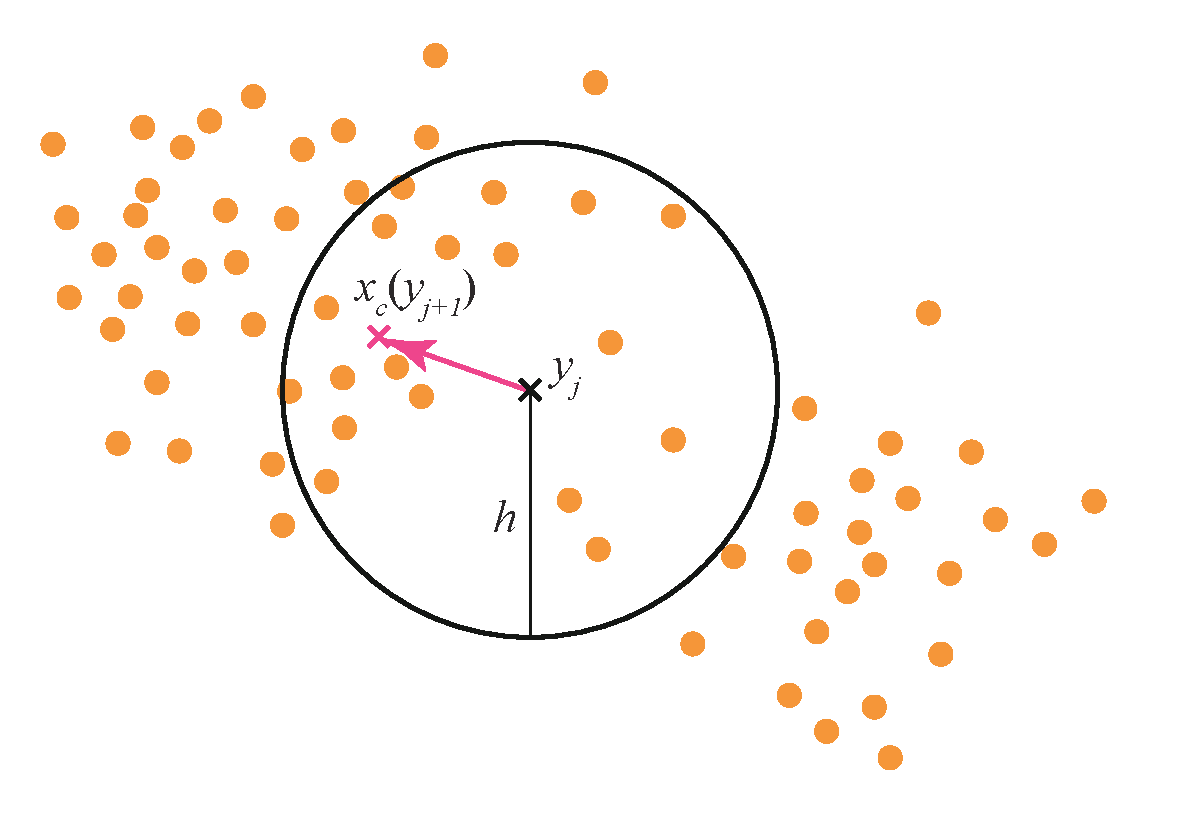
\includegraphics[width=0.7\linewidth]{img/mean-shift.pdf}
    \caption{Mean shiftによるクラスタリング}
    \label{fig:mean-shift}
  \end{center}
\end{figure}

Mean shiftを用いたクラスタリングは以下のように行う.
\begin{enumerate}
    \item 各点 $\vector{x}_i$にMean shiftを適用し,その収束位置 $\vector{x}_i^c$を計算する.
    \item 任意の2個の点$\vector{x}_i$, $\vector{x}_j$について,$\|\vector{x}_i^c - \vector{x}_j^c\| < \text{thereshold}$なら
      この2点を同じ極大点として同じクラスタとして扱う.
\end{enumerate}

Mean shiftは,$k$-meansと異なり,クラスタ数をあらかじめ指定する必要がない.

% 実験結果
\section{クラスタリング実験}

\subsection{実験環境}
実験にはPython3.5を用い,
機械学習のライブラリとしてTensorFlowを用いてアルゴリズムを実装した.

\subsection{精度の評価}
クラスタリング精度の評価はPythonのライブラリであるscilit-learnを用い,以下の3項目により行う.
\begin{description}
  \item[ARI; Adjusted Rand Index, 調整ランド指数]~\\
    クラスタの正解ラベルに対してクラスタリング結果の一致度を評価する指標.1に近づくほどよい結果.
  \item[NMI; Normalized Mutual Information, 正規化相互情報量]~\\
    相互情報量を正規化した尺度.
  \item[Purity]~\\
    生成されたクラスタがどれだけ多数派で占められているかを表す尺度
\end{description}

\subsection{X-meansによるクラスタリング}
\subsubsection{2次元のクラスタリング}

まず,2次元のデータのクラスタリング結果を比較する.
2次元空間に分散$\sigma^2=1$のGauss分布により生成した,クラスタあたりのサンプル数を500として5つのクラスタを生成し,
対数尤度関数,BIC, AIC, cAICによりクラスタリングを行った.

\tablenum{table:2dim}に100回クラスタリングを行ったときの,推定されたクラスタ数,ARI, NMI, Purityの平均値および
クラスタ数の分散値を示す.
また,\figurenum{fig:2dim}に2次元空間におけるクラスタリングの例を示す.

\begin{table}[htb]
  \centering
  \caption{2次元空間におけるクラスタリング結果}
  \label{table:2dim}
  \begin{tabular}{|c|c|c|c|c|} \hline
    情報量規準 & クラスタ数(分散) & ARI & NMI & Purity \\\hline
    BIC & 4.58 (0.9836) & 0.84458792 & 0.88281495 & 0.84458792\\
    cAIC & 4.55 (0.6475) & 0.85329139 & 0.89992544 & 0.85329139\\
    AIC & 4.69 (3.8739) & 0.83642236 & 0.88147442 & 0.83642236\\
    対数尤度関数 & 5.32 (10.236) & 0.85699618 & 0.91572100 & 0.85699618\\\hline 
  \end{tabular}
\end{table}

\begin{figure}[htbp]
  \begin{minipage}{0.5\hsize}
    \begin{center}
      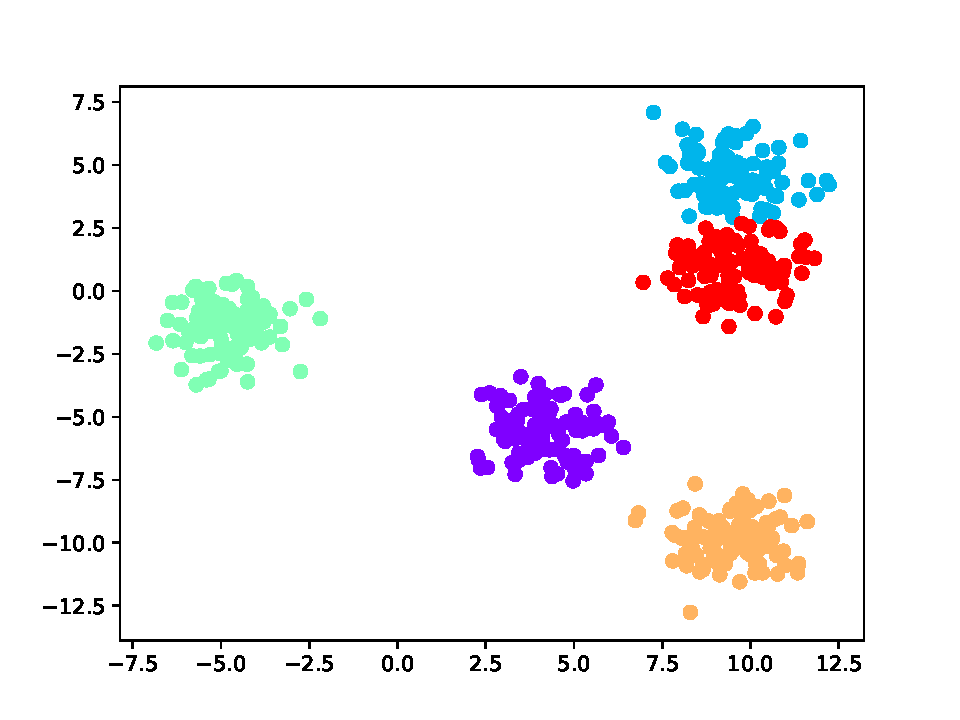
\includegraphics[width=0.9\linewidth]{./img/BIC_2.pdf}
      \caption{2次元空間のクラスタリング例}
      \label{fig:2dim}
    \end{center}
  \end{minipage}
  \begin{minipage}{0.5\hsize}
    \begin{center}
      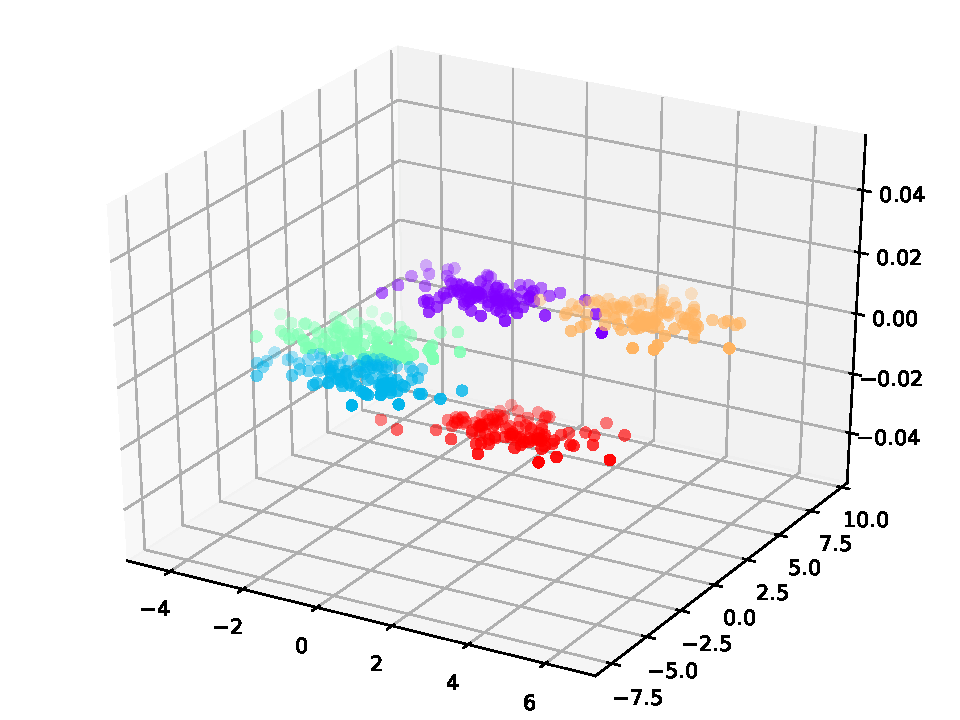
\includegraphics[width=0.9\linewidth]{./img/BIC_3.pdf}
      \caption{3次元空間のクラスタリング例}
      \label{fig:3dim}
    \end{center}
  \end{minipage}
\end{figure}

\subsubsection{3次元のクラスタリング}

3次元空間に分散$\sigma^2=1$のGauss分布により生成した,クラスタあたりのサンプル数を500として5つのクラスタを生成し,
対数尤度関数,BIC, AIC, cAICによりクラスタリングを行った.

\tablenum{table:3dim}に100回クラスタリングを行ったときの,推定されたクラスタ数,ARI,NMI,Purityの平均値および
クラスタ数の分散を示す.

また,\figurenum{fig:3dim}に2次元空間におけるクラスタリングの例を示す.

\begin{table}[htb]
  \centering
  \caption{3次元空間におけるクラスタリング結果}
  \label{table:3dim}
  \begin{tabular}{|c|c|c|c|c|} \hline
    情報量規準 & クラスタ数(分散) & ARI & NMI & Purity \\\hline
    BIC & 4.95 (0.0669) & 0.97179074 & 0.97913818 & 0.97179074\\
    cAIC & 4.92 (0.2313) & 0.96312702 & 0.97023920 & 0.96312702\\
    AIC & 4.88 (0.1443) & 0.95216819 & 0.96855698 & 0.95216819\\
    対数尤度関数 & 5.12 (4.1443) & 0.95731637 & 0.96541468 & 0.95731637\\\hline 
  \end{tabular}
\end{table}

% おわりに
\section{おわりに}

本研究では,いくつかの情報量規準を分割停止規準として採用してX-meansでクラスタ数推定を行った.
その結果,2次元空間における混合等方Gauss分布から生成したデータセットのクラスタリングにおいてはBICやcAICが,
3次元空間における混合等方Gauss分布から生成したデータセットのクラスタリングにおいてはBICが適していることがわかった.
2次元空間においてはAICを採用した場合,クラスタ数を過大に見積もってしまう問題が見受けられた.

以上より,混合等方Gauss分布により生成されたデータのクラスタリングを行う際は
BICを分割停止規準として採用することで適切なクラスタリングを行うことができると
言える.

今後は,AIC,cAIC,BIC以外の情報量規準を用いたクラスタリングや,
クラスタリング対象のデータを変更するなどして,それぞれのデータのクラスタリングに
最も適した情報量規準を探求していきたい.


% 参考文献
\section*{参考文献}
\begin{enumerate}
\renewcommand{\labelenumi}{\arabic{enumi})}
  \item James MacQueen et al.:
    Some methods for classification and analysis of multivariate observations,
    Proceedings of the fifth Berkeley symposium on mathematical statistics and probability,
    Vol. 1, No. 14, pp. 281--297 (1967).
  \item Akaike, H.: 
    Information theory and an extension of the maximum likelihood principle, 
    Proceedings of the 2nd International Symposium on Information Theory, 
    pp. 267-281 (1973).
  \item Dan Pelleg, Andrew W Moore, et al.:
    Xmeans: Extending K-means with Efficient Estimation of the Number of Clusters.,
    ICML, Vol. 1, pp. 727--734 (2000).
  \item Gideon Schwarz et al.:
    Estimating the dimension of a model,
    The annals of statistics, Vol. 6, No.2, pp. 461--464 (1978).
\end{enumerate}


\end{document}
